\documentclass[12pt,journal]{IEEEtran}

\usepackage[pdftex]{graphicx}
%\graphicspath{{../pdf/}{../jpeg/}}
\DeclareGraphicsExtensions{.pdf,.png,.jpg}
\usepackage{epstopdf}

\usepackage[cmex10]{amsmath}
\usepackage{multirow}
\usepackage{caption}

%\usepackage{mdwmath}
%\usepackage{mdwtab}
%\usepackage{array}
%\usepackage{eqparbox}

%\hyphenation{op-tical net-works semi-conduc-tor}

\begin{document}

\title{Stringless Guitar - Proyecto Final}
\author{Cuervo B., Nicolas y Horta C. Juan, D \\
 \{ncuervob,jdhortaca\} @unal.edu.co}

\markboth{Universidad Nacional de Colombia. Cuervo, Horta.~Final.~1, Junio~2012}%
{Shell \MakeLowercase{\textit{et al.}}: Bare Demo of IEEEtran.cls for Journals}

\maketitle

\begin{abstract}
\boldmath We've been working along the semester developing the course proyect: the stringless guitar. As we said in the first review, we've already reached the goal of generating sounds via pwm. From there, the effort was directed to generate the diferent notes of the guitar, and also, to emulate the guitar's sound. To accomplish this, FIR filters were very useful, as functions for the sorrounding wave (which give us the similarity of the guitar sound). The inputs of the system were send as interrupts via IRQ-GPIO using software developing; meanwhile, the synthesis of the sound is made as a hardware task to make it faster. An additional peripheral speaker is connected to a jack plug to hear the guitar, making it a digital "electro-acoustic look alike" device.
\end{abstract}

\begin{IEEEkeywords}
FPGA, guitar, PWM, sounds
\end{IEEEkeywords}
\section{Proponentes}
\begin{itemize}
	\item{Nicol\'as Cuervo Benavides. 261539}
	\item{Juan Daniel Horta. 260996}
\end{itemize}


\section{\'Area}
Electr\'onica Digital. Programaci\'on y desarrollo hardware - software.


\section{Introducci\'on}
En el presente escrito se presenta el desarrollo que ha tenido la realizaci\'on del proyecto final del curso: la \emph{Stringless Guitar}. Se ha trabajado a lo largo del semestre en la generaci\'on de sonidos a trav\'es del procesador; \'esto se ha logrado mediante una modulaci\'on por ancho de pulso (PWM por sus siglas en ingl\'es). Para \'esto se desarrollaron osciladores de diferentes frecuencias (para cada nota) con forma de diente de sierra (dado a que \'este tipo de onda es rico en arm\'onicos). Las entradas del sistema vienen de un tratamiento de se\~nal efectuado a rayos de luz interrumpidos, simulando as\'i las cuerdas de la guitarra; digitalmente se env\'ian a trav\'es del GPIO del procesador, y se toman c\'omo interrupciones. La salida del sistema es una se\~nal de audio, que es posible escuchar a trav\'es de unas bocinas externas. El desarrollo del proyecto de curso permiti\'o conocer las funcionalidades del procesador LM32, y c\'omo debe ser manipulado al entender su arquitectura. 


\section{Objetivos}

\textbf{General:} Presentar el dispositivo \emph{Stringless guitar} en funcionamiento.\\
\textbf{Especificos:}
\begin{itemize}
	\item{Generar se\~nales que puedan representar un sonido real mediante programaci\'on}
	\item{Filtrar la se\~nal generada con el fin de obtener un sonido semejante al producido en una guitarra}
	\item{Implementar la estructura de interfaz de usuario}
 \end{itemize}

\section{Cronograma}
El cronograma propuesto y las modificaciones realizadas a lo largo del desarrollo del proyecto se encuentran en el anexo 1.

\section{Comportamiento}
La idea consiste en emular una guitarra, s\'olo que prescindiendo de sus cuerdas. El dispositivo en vez de cuerdas cuenta con unos pares emisores-receptores de luz, de manera que una interrupci\'on en el trayecto del rayo lum\'inico envia una se\~nal al procesador, indic\'andole que debe generar el sonido. 
La forma f\'isica del dispositivo no difiere a el de una guitarra com\'un.

De cada par emisor-receptor el procesador recibe una se\~nal diferente, generando as\'i mismo un sonido a diferente frecuencia. Adem\'as se ha dispuesto de 4 pulsadores que emulan los trastes que al ser pulsados cambian la frecuencia del sonido generando, percibi\'endose una se\~nal m\'as aguda.
El flujo de datos que describe el sistema se aprecia en la fig. 1.
\begin{center}
	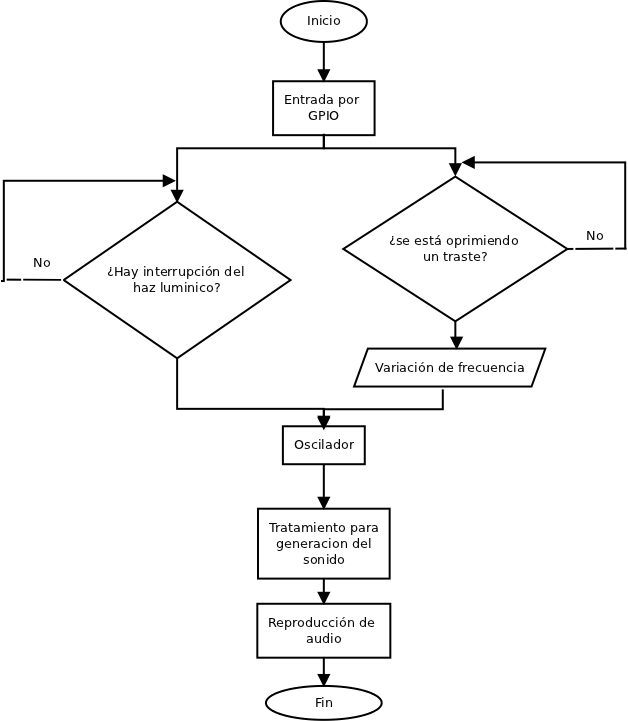
\includegraphics[scale=0.25]{flow1.png}
	\captionof{figure}{Diagrama de flujo de se\~nal}
\end{center}

\section{Especificaciones}  

\textbf{Temporales: }El dispositivo genera sonidos en tiempo real, como respuesta a una interrupci\'on f\'isica entre el emisor de luz y el receptor. Adem\'as, tambi\'en modifica la frecuencia del sonido emitido al pulsar los trastes; el delay que le toma al procesador efectuar esas operaciones no es perceptible al o\'ido humano.

\textbf{F\'isicas: }El dispositivo se ha instalado en un prototipo de madera con forma de guitarra c\'omo se pudo observar en la fig. 1, con unas dimensiones aproximadas de 56cm x 21cm x 9cm.

\textbf{Funcionales: }Las emisiones de luz se har\'an mediante lasers indicadores, mientras que fotoceldas tendr\'an la funci\'on de receptores. El estado estable del dispositivo consiste en un flujo ininterrumpido entre los emisores y los receptores. Una interrupci\'on efectuada sobre el haz de luz envia una sen\~al al procesador y genera el sonido. Adem\'as, a partir de pulsadores que emulan los trastes se obtienen variaciones en los osciladores, generando sonidos m\'as agudos al ser pulsados.

\textbf{El\'ectricas: }El dispositivo se alimentar\'a con una bater\'ia de 3.7v.

\section{Arquitectura del sistema}
Las tareas del dispositivo se dividen en la manera en que son instanciadas, ya sea hardware o software. \'Estas son:
\subsection*{Tareas hardware}
El criterio principal para determinar las tareas que se deben efectuar por medio de hardware es b\'asicamente la velocidad. Dado a que se est\'a generando audio en tiempo real, es requerido que \'este se obtenga sin demora al momento en que efect\'ua la solicitud. La instanciaci\'on hardware permite generar esta interfaz necesaria para que los delays de procesamiento no sean notorios para el usuario. Las tareas efectuadas en este apartado son:
\begin{itemize}
	\item Recepci\'on de las se\~nales externas desde los pulsadores
	\item Generaci\'on del oscilador y su tratamiento para obtener los sonidos
	\item Reproducci\'on del sonido generado.
\end{itemize}

\subsection*{Tareas software}
Las tareas efectuadas en software son meramente de control. La programaci\'on software fue vital para manejar los procesos de interrupciones a partir de las entradas externas, as\'i como el control del proceso de generaci\'on de audio en general.
\begin{itemize}
	\item Control general de perif\'ericos y generaci\'on de audio
\end{itemize}

\section{Estructura}
B\'asicamente la operaci\'on del dispositivo puede dividirse en etapas, caracterizadas por la funci\'on que ejercen dentro del proceso. Estas etapas se pueden apreciar en la fig. 2.

\begin{center}
	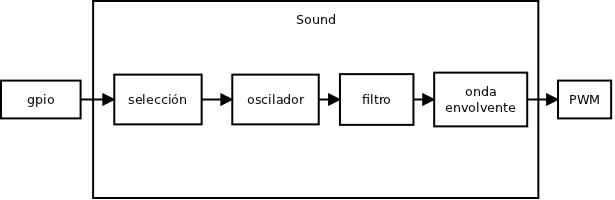
\includegraphics[scale=0.25]{bloques.png}
	\captionof{figure}{Diagrama de bloques del dispositivo}
\end{center}

Siguiendo el flujo de datos de izquierda a derecha en la fig. 2, el primer bloque corresponde a la entrada de datos mediante el perif\'erico de \emph{entradas y salidas de prop\'osito general} (GPIO, por sus siglas en ingl\'es). En \'este perif\'erico se toman las entradas externas que provienen de las interrupciones en el haz de luz o de los pulsadores. Estas entradas van al m\'odulo de \emph{Sound} donde se sintetiza toda la parte de generaci\'on de audio. C\'omo se puede apreciar \'este segmento se compone del bloque de la selecci\'on, el oscilador, el filtrado y la onda envolvente.

\subsection*{Selecci\'on}
\begin{center}
	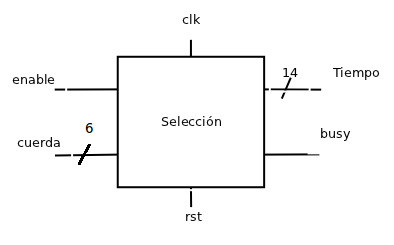
\includegraphics[scale=0.35]{seleccion.png}
	\captionof{figure}{Entrada/salida del m\'odulo de selecci\'on}
\end{center}

B\'asicamente, c\'omo su nombre lo indica, este m\'odulo tiene la funci\'on de seleccionar las cuerdas de manera que el oscilador tenga el par\'ametro correspondiente a partir de las entradas recibidas del GPIO.

\subsection*{Oscilador}
\begin{center}
	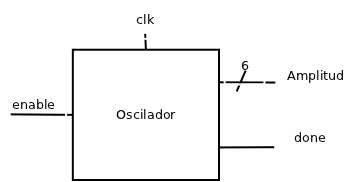
\includegraphics[scale=0.35]{oscilador.png}
	\captionof{figure}{Entrada/salida del m\'odulo del oscilador}
\end{center}

En este m\'odulo se crea por medio de instanciaci\'on hardware una señal de la forma diente de sierra. \'Esto se hace mediante un contador. El m\'odulo internamente tiene unos par\'ametros que determinan su frecuencia; sin embargo estos son elegidos a partir de la señal de enable proveniente del proceso de selecci\'on. 

\subsection*{Filtros}
\begin{center}
	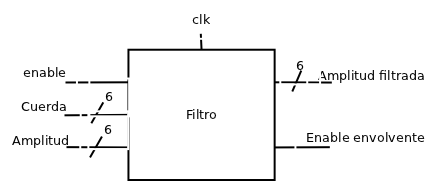
\includegraphics[scale=0.35]{filtro.png}
	\captionof{figure}{Entrada/salida del m\'odulo del filtro}
\end{center}

La funci\'on de este m\'odulo es limitar los valores de frecuencia de la señal obtenida en el oscilador, de manera que los cambios de amplitud no sean abruptos. Para esta secci\'on se ha decidido utilizar filtros FIR, dado a que requieren menos recursos para operar que su contraparte IIR. Los filtros FIR operan como se aprecia en la fig. 6. \par


\begin{center}
	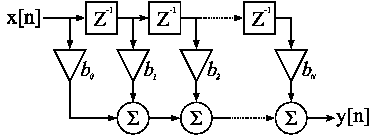
\includegraphics[scale=0.75]{fir.png}
	\captionof{figure}{Diagrama de un filtro FIR [1]}
\end{center}

Lo interesante de estos filtros es que no tienen memoria; es decir, su comportamiento depende \'unicamente de la entrada actual y no de valores pasados, de manera que su respuesta siempre es finita.

F\'isicamente estos filtros son los que permiten la semejanza a el sonido de la guitarra. Dado a que es un filtro de alto orden (10), as\'i mismo se requieren coeficientes para su funcionamiento. Estos valores de coeficientes al ser variados arrojan un sonido m\'as suave o m\'as fuerte.
 \subsection*{Onda envolvente}
\begin{center}
	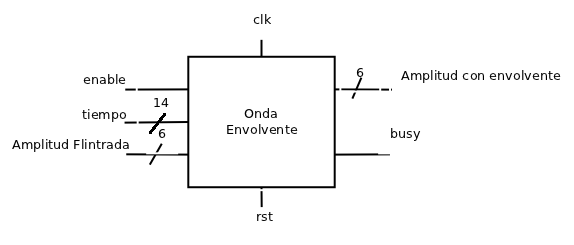
\includegraphics[scale=0.35]{envolvente.png}
	\captionof{figure}{Entrada/salida del m\'odulo de la onda envolvente}
\end{center}

Este m\'odulo se encarga de emular la duraci\'on e intensidad del sonido de una guitarra. Es fácil identificar que, al tocar una cuerda, la amplitud de la onda de audio crece r\'apidamente hasta su valor m\'aximo, mantiene una amplitud de la nota y luego cae en el tiempo. \'Este proceso se ha estudiado bastante en el \'ambito de la generaci\'on de sonidos, y se han identificado las etapas que tiene el s\'onido al ser generado en: attack, decay, sustain, release.
\begin{center}
	
\includegraphics[scale=0.25]{ADSR.png}
	\captionof{figure}{Forma de onda envolvente, con sus respectivas etapas}
\end{center}

Para cada etapa presente en la fig. 8 se desarroll\'o un submodulo, variando la amplitud de la señal filtrada y de esta manera generando semejanza a el decaimiento temporal de una nota al ser tocada en una guitarra.

\subsection*{PWM}
PWM [3] es la sigla en ingl\'es de modulaci\'on por anchura de pulsos (pulse-width modulation), y es una t\'ecnica en la que se modifica, c\'omo su nombre lo indica, el ancho del pulso de una señal peri\'odica; este ancho se denomina ciclo de trabajo, tom\'andose su medida en relaci\'on con el  periodo de la se\~nal.
\begin{figure}[h]
\centering
 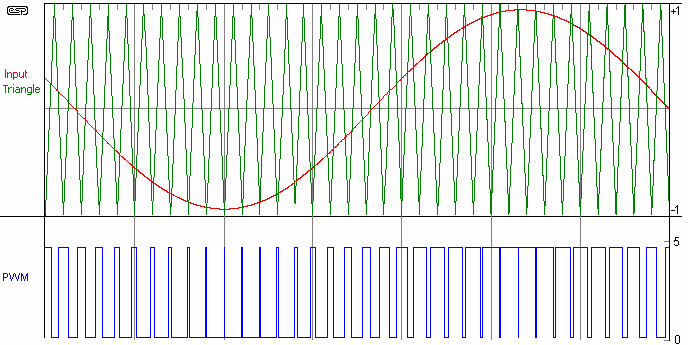
\includegraphics[scale=0.5]{PWM1.png}
        \caption{PWM}
\end{figure}

Con \'este m\'odulo lo que se busca es generar señales a diferentes frecuencias, siendo las frecuencias elegidas las que caracterizan las notas determinadas. Luego, a la salida de la fpga mediante un filtro suavizar la señal de manera que sea audible.

 \begin{center}
	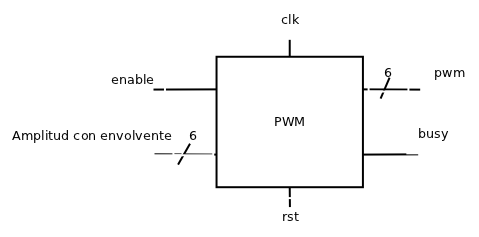
\includegraphics[scale=0.25]{PWM.png}
	\captionof{figure}{M\'odulo de la PWM}
\end{center}

C\'omo parte final de la generaci\'on de audio, se utiliz\'o la modulaci\'on por ancho de pulso para efectuar una conversi\'on an\'alogica/digital sin necesidad de un ADC extra. En \'este m\'odulo, el ancho del ciclo de trabajo de cada pulso est\'a relacionado con la amplitud de la señal de entrada; es decir, la amplitud de la señal luego de pasar por la onda envolvente. De esta manera se obtiene a la salida del sistema una variaci\'on perceptible al conectar una bocina; \'esta señal de pwm es la salida principal del dispositivo. La conexi\'on de la salida del dispositivo es directa a unas bocinas externas, c\'omo se especificar\'a posteriormente en este mismo escrito.

\section{Comunicaci\'on Wishbone}
La intercomunicaci\'on entre m\'odulos y tareas hardware/software se realiza utilizando el protocolo wishbone. Para lograr la comunicaci\'on es preciso determinar jerarqu\'as entre bloques del procesador. De esta manera, se dispone de un maestro que es la unidad de procesamiento CPU, y de dos esclavos: GPIO y el m\'odulo Sound. El diagrama de bloques del proceso se aprecia en la fig. 
\begin{center}
	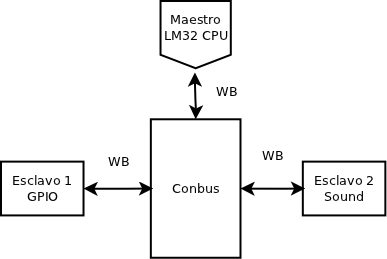
\includegraphics[scale=0.3]{wb.png}
	\captionof{figure}{Intercomunicaci\'on utilizando protocolo wishbone}
\end{center}

\section{Montaje}
Para el montaje f\'isico del dispositivo se desarroll\'o un circuito al cual se conectan los sensores lum\'inicos y se env\'ian a la fpga. El esquem\'atico del diseño se aprecia en el Anexo 2. Las sen\~nales obtenidas de los sensores son anal\'ogicas, de manera que fue necesario digitalizarlas. Con este fin, se vali\'o del uso de una Schmitt trigger.
\begin{center}
	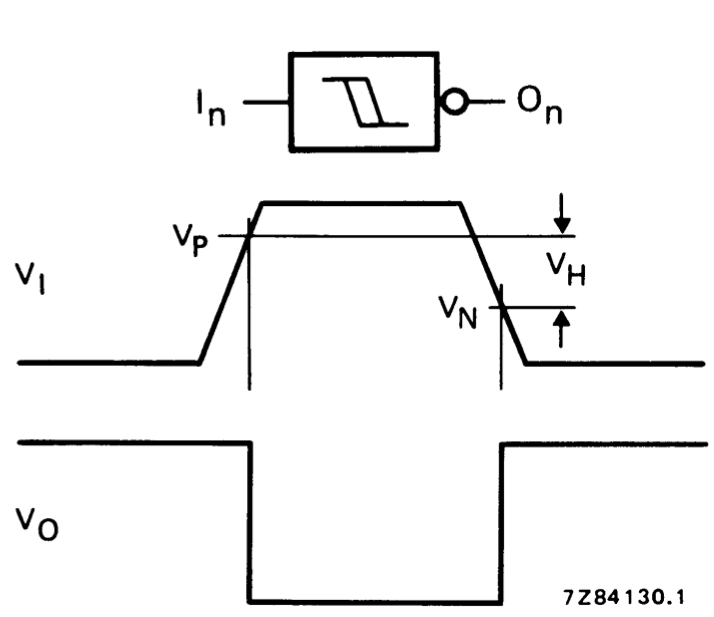
\includegraphics[scale=0.3]{schmitt.png}
	\captionof{figure}{Formas de onda de entrada y salida de una compuerta Schmitt trigger}
\end{center}

El funcionamiento de esta compuerta es bastante sencillo: al sobrepasarse un nivel de tension de "gatillo", la compuerta arroja a la salida un nivel alto. De manera an\'aloga, al encontrarse a una tensi\'on m\'as baja, la compuerta arroja una salida de nivel bajo. B\'asicamente digitaliza la señal a 1 bit de informaci\'on. De \'esta manera, esa se\~nal digital funciona c\'omo interruptor que va al GPIO. \par

Luego del tratamiento de se\~nal, la salida del m\'odulo pwm es adquirida a trav\'es de un conector Jack de audio para ser conectada a unas bocinas externas; as\'i se evita el tener que adicionar una etapa de amplificaci\'on y filtrado de la sen\'al.

El dise\~no de la pcb se realiz\'o utilizando \emph{Proteus}. El resultado se aprecia en la fig. 13.
\begin{center}
	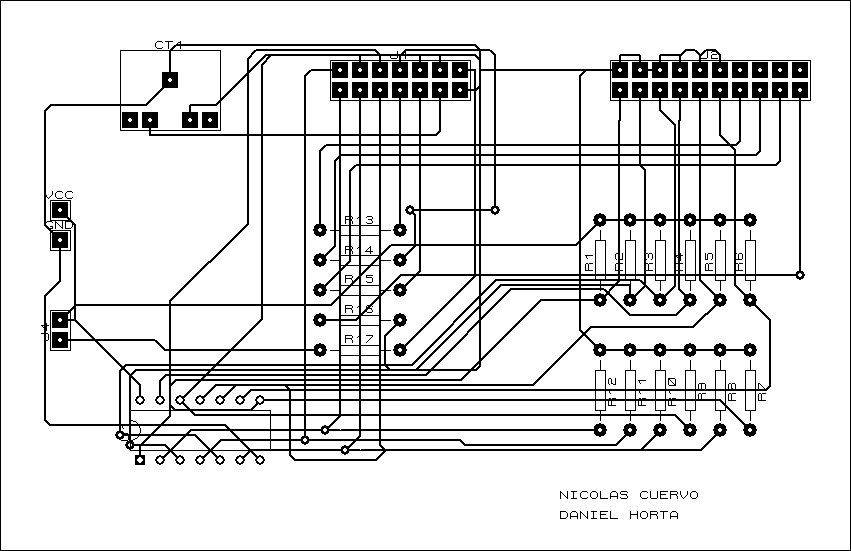
\includegraphics[scale=0.25]{1.png}
	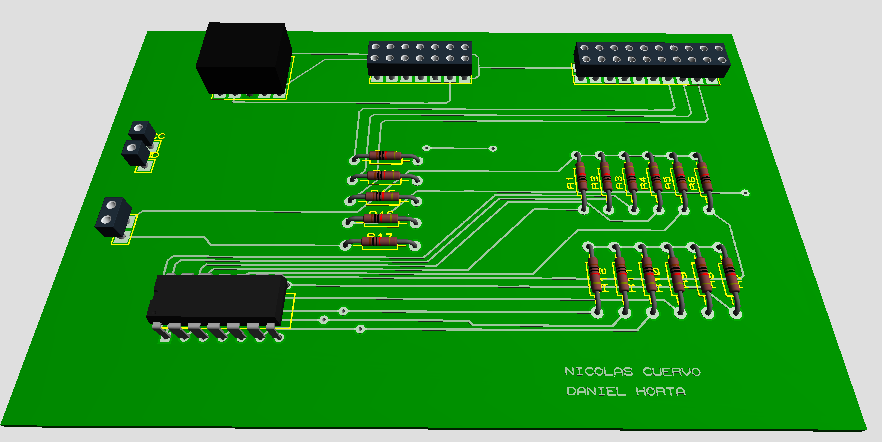
\includegraphics[scale=0.25]{3d.png}
	\captionof{figure}{Circuito Impreso}
\end{center}
 
C\'omo producto final se instal\'o el dispositivo desarrollado en una guitarra mediana. 

\section{An\'alisis de costos}
El an\'alisis de costos detallado se encuentra en el anexo 3.

\section{Conclusiones}
\begin{itemize}
	\item El producto obtenido representa un desarrollo que se ha venido realizando a lo largo del curso, realizando un manejo de la arquitectura de los procesadores, más especificamente del LM32. Más que la generaci\'on de audio, el proyecto tiene un enfoque de innovaci\'on, donde prima la manera original de presentar dispositivos originales utilizando la tecnolog\'ia existente.
	\item El desarrollo de un elemento de ingenier\'ia no se limita a lo obtenido en una sesi\'on de programaci\'on. Un dispositivo que sea aceptado en la industria debe tener tanto un alto nivel de ingenier\'ia de desarrollo como una interfaz de usuario llamativa y sencilla. Para este proyecto se imprimi\'o un gran esfuerzo en lograr un elemento que sea llamativo al p\'ublico en general, elemento que representa una gran fracci\'on del segmento objetivo en la industria profesional.
\end{itemize}

\section{Proyectos futuros}
El producto final es un elemento bastante llamativo, pero podr\'ian ser aplicadas nuevas tecnolog\'ias para optimizarlo. Al introducir t\'ecnicas de sintesis de audio m\'as avanzadas se podr\'ia emular mejor el sonido de la guitarra. Adem\'as, el uso de sensores m\'as sofisticados tanto para las cuerdas c\'omo para los trastes podr\'ian dar v\'ia a alternativas interesantes de desarrollo musical digital.  

\begin{thebibliography}{1}


\bibitem{IEEEhowto:C\'adiz}
R.~C\'adiz, \emph{Filtros FIR}, [En L\'inea] Disponible en:"http://www.rodrigocadiz.com/imc/html/Filtros\_FIR.html" Fecha de consulta: 13-06-2012

\bibitem{IEEEhowto:Taigen}
H.~Taigen, \emph{Musical Blocks}, [En L\'inea] Disponible en:"http://people.ece.cornell.edu/land/courses/ece4760/FinalProjects\\/s2009/jvt6\_th389/jvt6\_th389/finalproject.html" Fecha de consulta: 6-06-2012

\bibitem{IEEEhowto:Stanford}
S. ~Vanheesbeke, \emph{Swapping bits improves performance of FPGA-PWM counter}, EDN Europe: Electronics DEsign, Strategy, News [En L\'inea] Disponible en:"Swapping bits improves performance of FPGA-PWM counter" Fecha de consulta: 07-05-2012

\end{thebibliography}


\end{document}



